% =============================================================================
%  UI System
% =============================================================================
\section{UI System}
\label{sec:ui_system}

\subsection{Overview}

The graphical front-end is a \emph{pygame}-based desktop application running
at a fixed resolution of $900 \times 680$ pixels and locked to 60 frames per
second.
It exposes the solver framework interactively through three operating modes —
manual play, step-by-step solver visualisation, and CNF knowledge-base
exploration — all sharing a single window layout.

The UI is structured around four concerns that are kept deliberately separate:

\begin{enumerate}
  \item \textbf{State} (\texttt{GameState}) — a single flat dataclass that
        holds every mutable flag; owned exclusively by the main thread.
  \item \textbf{Input} (\texttt{InputHandler}) — translates pygame events into
        state mutations and calls to \texttt{GameApplication}.
  \item \textbf{Rendering} (\texttt{CompositeRenderer} and sub-renderers) —
        reads state and draws every frame; never mutates state.
  \item \textbf{Application controller} (\texttt{GameApplication}) — runs the
        event loop, owns the clock, and coordinates the other three.
\end{enumerate}

% =============================================================================
\subsection{Window Layout}
\label{sec:ui_layout}

\begin{figure}[h]
  \centering
  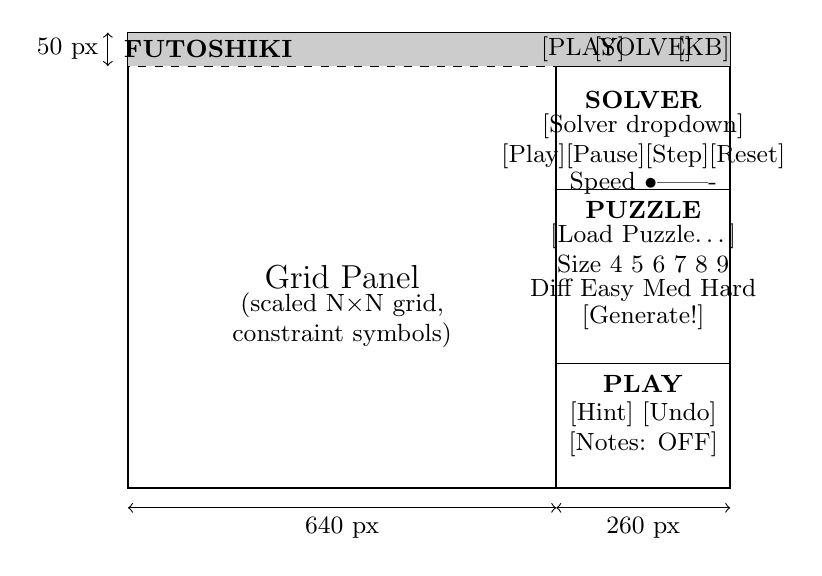
\begin{tikzpicture}[scale=0.85, every node/.style={font=\small}]
    % Outer window
    \draw[thick] (0,0) rectangle (9, 6.8);

    % Title bar
    \fill[gray!40] (0,6.3) rectangle (9, 6.8);
    \node at (1.2, 6.55) {\textbf{FUTOSHIKI}};
    \node at (6.8, 6.55) {[PLAY]};
    \node at (7.7, 6.55) {[SOLVE]};
    \node at (8.6, 6.55) {[KB]};

    % Grid area
    \draw[dashed] (0,0) rectangle (6.4, 6.3);
    \node at (3.2, 3.15) {\large Grid Panel};
    \node[align=center] at (3.2, 2.5) {(scaled N$\times$N grid,\\constraint symbols)};

    % Side panel separator
    \draw[thick] (6.4, 0) -- (6.4, 6.3);

    % Solver panel
    \draw (6.4, 4.45) rectangle (9, 6.3);
    \node[align=left] at (7.7, 5.8) {\textbf{SOLVER}};
    \node[align=left] at (7.7, 5.4) {[Solver dropdown]};
    \node[align=left] at (7.7, 4.95) {[Play][Pause][Step][Reset]};
    \node[align=left] at (7.7, 4.55) {Speed $\bullet$-------};

    % Puzzle panel
    \draw (6.4, 1.85) rectangle (9, 4.45);
    \node[align=left] at (7.7, 4.15) {\textbf{PUZZLE}};
    \node[align=left] at (7.7, 3.75) {[Load Puzzle\ldots]};
    \node[align=left] at (7.7, 3.35) {Size 4 5 6 7 8 9};
    \node[align=left] at (7.7, 2.95) {Diff Easy Med Hard};
    \node[align=left] at (7.7, 2.55) {[Generate!]};

    % Play panel
    \draw (6.4, 0) rectangle (9, 1.85);
    \node[align=left] at (7.7, 1.55) {\textbf{PLAY}};
    \node[align=left] at (7.7, 1.1) {[Hint] [Undo]};
    \node[align=left] at (7.7, 0.65) {[Notes: OFF]};

    % Dimension annotations
    \draw[<->] (0,-0.3) -- (6.4,-0.3) node[midway, below] {640 px};
    \draw[<->] (6.4,-0.3) -- (9,-0.3) node[midway, below] {260 px};
    \draw[<->] (-0.3, 6.3) -- (-0.3, 6.8) node[midway, left] {50 px};
  \end{tikzpicture}
  \caption{Window layout in PLAY/SOLVE mode.  In KB mode the entire side panel
           is replaced by the CNF knowledge-base viewer.}
  \label{fig:ui_layout}
\end{figure}

\subsubsection{Coordinate System}

All layout constants live in \texttt{ui/layout.py} and are computed once at
module load time.
\texttt{grid\_geometry(N)} is the only dynamic function: it computes the
cell size and gap for an $N \times N$ grid by taking the minimum of the
width-constrained and height-constrained cell size and centering the result
inside the 640-pixel grid area.

\begin{align*}
  \text{cell\_size} &= \min\!\left(
    \frac{W_{\text{grid}} - 2P - (N-1)g}{N},
    \frac{H_{\text{grid}} - 2P - (N-1)g}{N}
  \right) \\
  g &= 18\ \text{px} \quad (\text{constraint symbol gap}) \\
  P &= 30\ \text{px} \quad (\text{outer padding})
\end{align*}

Two derived helpers map logical coordinates to pixel rects:

\begin{description}
  \item[\texttt{cell\_rect(i, j, grid\_rect, cell\_size, gap)}]
    Returns the pixel \texttt{pygame.Rect} for cell $(i,j)$.
  \item[\texttt{h\_gap\_rect} / \texttt{v\_gap\_rect}]
    Return the pixel rect of the inter-cell gap where a constraint symbol
    is drawn.
\end{description}

% =============================================================================
\subsection{Theme System}
\label{sec:ui_theme}

\texttt{ui/theme.py} centralises all visual constants.
Renderers import \texttt{ui.theme as T} and reference symbols directly
(\texttt{T.CLR\_CELL\_ERROR}, \texttt{T.font("hud\_label")}, etc.).

\subsubsection{Colour Palette}

\begin{table}[h]
  \centering
  \caption{Cell background colours and their semantics.}
  \label{tab:theme_colours}
  \begin{tabular}{lll}
    \toprule
    Constant & RGB & Meaning \\
    \midrule
    \texttt{CLR\_CELL\_DEFAULT}   & (255, 255, 255) & Empty, user-editable cell \\
    \texttt{CLR\_CELL\_GIVEN}     & (210, 210, 205) & Pre-filled clue \\
    \texttt{CLR\_CELL\_SELECTED}  & (180, 210, 255) & Currently focused cell \\
    \texttt{CLR\_CELL\_ERROR}     & (255, 180, 180) & Constraint violation \\
    \texttt{CLR\_CELL\_SOLVER}    & (180, 220, 255) & Value placed by solver \\
    \texttt{CLR\_CELL\_BACKTRACK} & (255, 200, 130) & Backtrack flash (orange) \\
    \texttt{CLR\_CELL\_SOLVED}    & (180, 255, 190) & Final solved state (green) \\
    \texttt{CLR\_CELL\_KB\_HL}    & (255, 210,  80) & KB-mode hover highlight \\
    \bottomrule
  \end{tabular}
\end{table}

\subsubsection{Font Hierarchy}

Fonts are lazily initialised by \texttt{init\_fonts()} after \texttt{pygame.init()}.
The font size scales with the grid: \texttt{cell\_font(N)} returns a 32 pt bold
font for $N \le 5$, 24 pt for $N \le 7$, and 18 pt for $N \ge 8$.
Note fonts follow the same breakpoints (11 pt / 9 pt) to keep pencil marks
legible even at small cell sizes.

% =============================================================================
\subsection{Renderer Architecture}
\label{sec:ui_renderers}

\subsubsection{BaseRenderer and Composite Pattern}

\texttt{ui/base.py} defines a minimal abstract class:
\begin{lstlisting}[language=Python]
class BaseRenderer(ABC):
    @abstractmethod
    def render(self, surface: pygame.Surface, state: GameState) -> None: ...
\end{lstlisting}

\texttt{CompositeRenderer} holds three sub-renderers and delegates in draw
order:

\begin{enumerate}
  \item \textbf{\texttt{GridRenderer}} — cells, values, notes, backtrack flash,
        KB highlights, notification overlay, domain tooltip.
  \item \textbf{\texttt{ConstraintRenderer}} — inequality symbols in inter-cell
        gaps.
  \item \textbf{\texttt{HudRenderer}} — title bar, mode tabs, and the entire
        right-hand side panel (or KB panel in KB mode), plus all modal overlays
        drawn on top.
\end{enumerate}

Renderers are \emph{stateless} — they read \texttt{GameState} and draw, but
never modify it.
All mutable output (hit-test rects) is written into \texttt{state.\_hud\_rects},
a dict that is cleared and rebuilt every frame by \texttt{HudRenderer}.
This means \texttt{InputHandler} can read click targets from the same place
the renderer just wrote them without any synchronisation.

\subsubsection{GridRenderer}

\textbf{Cell drawing} is the innermost loop.
For each cell $(i,j)$, the renderer applies a priority chain to determine the
background colour:

\begin{enumerate}
  \item Given (clue) cell → \texttt{CLR\_CELL\_GIVEN}
  \item Error (in \texttt{board.errors}) → \texttt{CLR\_CELL\_ERROR}
  \item Backtrack flash (in \texttt{state.backtrack\_timers}) →
        linear interpolation between \texttt{CLR\_CELL\_BACKTRACK} (orange) and
        \texttt{CLR\_CELL\_DEFAULT} (white), controlled by the remaining timer
        fraction $t/0.5$
  \item Solve succeeded and cell filled → \texttt{CLR\_CELL\_SOLVED}
  \item Solver-placed (in \texttt{state.solver\_cells}) →
        \texttt{CLR\_CELL\_SOLVER}
  \item Selected → \texttt{CLR\_CELL\_SELECTED}
  \item Default → \texttt{CLR\_CELL\_DEFAULT}
\end{enumerate}

\textbf{Shake animation} for invalid note attempts: when a key press is blocked
(the value already exists in the row or column), \texttt{state.shake\_timers}
records a 0.4 s countdown for that cell.
The renderer reads the remaining time and applies a horizontal pixel offset:
\[
  \Delta x = \left\lfloor \sin(t_\text{elapsed} \cdot 45) \cdot 6 \cdot
             \frac{t_\text{remaining}}{0.4} \right\rfloor
\]
producing a decaying sinusoidal oscillation that visually indicates rejection.

\textbf{Pencil marks} are drawn in a sub-grid inside the cell.
Values are arranged in rows of $\max(3, \lfloor N/2 \rfloor + 1)$ columns,
each occupying a $(\text{cell\_w}/\text{cols}) \times (\text{cell\_h}/\text{rows})$
sub-cell.

\textbf{KB mode highlights}: when \texttt{state.mode == AppMode.KB}, the
renderer checks \texttt{state.kb\_hovered\_clause} (rule hover) or
\texttt{state.kb\_hovered\_lit} / \texttt{state.kb\_selected\_lit} (fact hover
or click-pin).
Cells referenced by the literal/clause receive a semi-transparent amber
overlay (\texttt{CLR\_CELL\_KB\_HL}, alpha=160) drawn with
\texttt{pygame.SRCALPHA}.

\textbf{Domain tooltip}: in KB mode, hovering the mouse over a grid cell draws
a small pop-up showing the cell coordinates and either its fixed value (if
given) or its naive domain (values not yet placed in the same row/column).

\subsubsection{ConstraintRenderer}

Iterates \texttt{puzzle.h\_constraints} and \texttt{puzzle.v\_constraints} and
draws \texttt{<}, \texttt{>}, \texttt{\^}, or \texttt{v} in the appropriate
gap rect.
In KB mode, a constraint symbol is highlighted (amber background, coloured
text) when:
\begin{itemize}
  \item The hovered literal is a \texttt{LessH}/\texttt{GreaterH}/\texttt{LessV}/\texttt{GreaterV}
        fact naming this exact constraint; or
  \item The hovered clause contains a literal that directly names this
        constraint, \emph{or} contains \texttt{Val}/\texttt{NotVal} literals
        that reference both cells connected by the constraint
        (covering axioms A5–A8 and A16 which reference only cell values, not
        the constraint predicate directly).
\end{itemize}

\subsubsection{HudRenderer}

\textbf{Hit-test rect registration.} Every button, slider, row, and tab is
drawn using \texttt{\_draw\_button()} (a helper that applies normal/hover/active/
disabled colouring) and its \texttt{pygame.Rect} is immediately stored into
\texttt{state.\_hud\_rects} under a string key.
\texttt{InputHandler} reads these rects for collision testing on the next
click event.
Because rects are reset each frame, a button that disappears (e.g.\ the play
button when no puzzle is loaded) automatically stops being clickable.

\textbf{Solver panel} (185 px tall):
\begin{itemize}
  \item \emph{Solver selector}: a drop-down button showing the current
        solver's display name.
        When active, a floating overlay lists all ten solvers as clickable
        rows; drawn on top of everything else so it visually overlaps adjacent
        panels.
  \item \emph{Control buttons}: Play / Pause / Step / Reset, each with a
        corresponding key in \texttt{state.\_hud\_rects}.
        Greyed out (disabled state) when \texttt{mode != SOLVE}.
  \item \emph{Speed slider}: a horizontal track with a draggable thumb;
        maps pixel position to a value in $[1.0, 20.0]$ steps/second.
  \item \emph{Stats display}: node count, elapsed ms, backtrack count, and a
        status line (\emph{Solving\ldots} / \emph{Paused} / \emph{Solved!} /
        \emph{No solution}).
\end{itemize}

\textbf{Puzzle panel} (265 px tall):
\begin{itemize}
  \item \emph{Load Puzzle\ldots}: opens the puzzle list overlay (a modal card
        centred over the grid area listing all 24 benchmark puzzles with
        name, size, and difficulty).
  \item \emph{Generate}: size radio buttons (4–9) and difficulty radio buttons
        (Easy / Medium / Hard), then a [Generate!] button that spawns a daemon
        thread and shows a \emph{Generating\ldots} spinner overlay.
\end{itemize}

\textbf{Play panel} (remaining height):
\begin{itemize}
  \item \emph{Hint}: calls \texttt{board.get\_hint()} (AC-3 domain reduction;
        returns the first singleton-domain cell) and applies the result.
  \item \emph{Undo}: calls \texttt{board.undo()}.
  \item \emph{Notes: ON/OFF}: toggles \texttt{state.notes\_mode}; button
        colour changes to indicate active state.
\end{itemize}

\textbf{KB panel} (full side panel height, shown when \texttt{mode == KB}):
\begin{itemize}
  \item Header with total/unit/binary/longer clause counts.
  \item \emph{FACTS / RULES} tab toggle.
  \item Scrollable list of unit clauses (FACTS view) or multi-literal clauses
        (RULES view), with \texttt{\^}/\texttt{v} scroll buttons and a
        position indicator.
  \item Each fact row has a \texttt{[?]} button that pins the explanation in
        the info box below.
  \item \emph{Info/explanation box} at the bottom: shows a human-readable
        description of the hovered or pinned fact/clause (e.g.\ ``Cell (2,3)
        cannot hold value 4.'').
  \item \emph{CNF Reference popup}: clicking \texttt{[?]} in the header opens
        a modal card over the grid with a scrollable reference describing all
        predicates and axiom groups.
\end{itemize}

% =============================================================================
\subsection{Input System}
\label{sec:ui_input}

\subsubsection{Event Dispatch Priority}

\texttt{InputHandler.handle\_click()} resolves click targets in a strict
priority order:

\begin{enumerate}
  \item KB reference popup (if open) — consumes all clicks.
  \item Puzzle list overlay (if open) — row selection or close.
  \item Generate dialog (if open) — blocks all input while generating.
  \item Solver dropdown (if open) — selection or dismiss.
  \item Mode tab bar (PLAY / SOLVE / KB).
  \item Solve controls (only when \texttt{mode == SOLVE}).
  \item Speed slider.
  \item Puzzle panel buttons and radio groups.
  \item Play panel buttons.
  \item KB mode: panel navigation and fact interaction.
  \item Grid cell click (only when \texttt{mode == PLAY}).
\end{enumerate}

Each handler returns immediately after processing so lower-priority targets
cannot be accidentally triggered by the same click.

\subsubsection{Keyboard Bindings}

\begin{table}[h]
  \centering
  \caption{Keyboard bindings.}
  \label{tab:keybindings}
  \begin{tabular}{lll}
    \toprule
    Key & Mode & Action \\
    \midrule
    \texttt{Esc}          & Any     & Close topmost modal overlay \\
    \texttt{F1}           & Any     & Switch to PLAY mode \\
    \texttt{F2}           & Any     & Switch to SOLVE mode \\
    \texttt{1}–\texttt{N} & PLAY    & Enter value (or toggle note in notes mode) \\
    \texttt{0}/\texttt{Backspace}/\texttt{Delete} & PLAY & Clear selected cell \\
    Arrow keys            & PLAY    & Move cell selection \\
    \texttt{Ctrl+Z}       & PLAY    & Undo last edit \\
    \texttt{N}            & PLAY    & Toggle notes mode \\
    \texttt{Space}        & SOLVE   & Toggle play/pause \\
    \texttt{Right arrow}  & SOLVE   & Advance one step \\
    \texttt{R}            & SOLVE   & Restart solver \\
    Mouse wheel           & KB/List & Scroll fact/rule list or popup \\
    \bottomrule
  \end{tabular}
\end{table}

\subsubsection{Hover Tracking}

In KB mode, every \texttt{MOUSEMOTION} event calls
\texttt{\_update\_kb\_hover()}, which:
\begin{enumerate}
  \item Scans \texttt{state.\_hud\_rects["\_kb\_fact\_rows"]} to find
        the hovered fact literal.
  \item Scans \texttt{state.\_hud\_rects["\_kb\_rule\_rows"]} to find
        the hovered clause.
  \item Iterates all $N^2$ cell rects to find the hovered grid cell (for the
        domain tooltip).
\end{enumerate}

The state fields \texttt{kb\_hovered\_lit}, \texttt{kb\_hovered\_clause}, and
\texttt{kb\_hovered\_cell} are updated in place.
On the next frame, both \texttt{GridRenderer} and \texttt{ConstraintRenderer}
read these fields to draw the cell and symbol highlights — a clean
read-only renderer / write-only input handler split.

% =============================================================================
\subsection{Solve Visualisation}
\label{sec:ui_solve}

\subsubsection{Step Emission}

When \texttt{GameApplication.\_start\_solve()} is called, \texttt{start\_solve()}
in \texttt{app/solve\_worker.py}:

\begin{enumerate}
  \item Resets all visualisation state (\texttt{GameState.reset\_solve\_state()}).
  \item Builds a closure \texttt{on\_step(grid\_snapshot, is\_backtrack=False)}.
  \item Launches a daemon thread that calls \texttt{solver.solve(puzzle,
        on\_step=on\_step)}.
  \item Sets \texttt{state.is\_playing = True} so animation begins immediately.
\end{enumerate}

\texttt{on\_step} performs three tasks:

\begin{enumerate}
  \item \textbf{Backtrack detection.}
        If the caller does not set \texttt{is\_backtrack=True} explicitly,
        the function detects a backtrack by comparing
        \texttt{np.count\_nonzero(grid\_snapshot)} against the previous grid.
        A decrease in filled cells signals a backtrack; the counter
        \texttt{\_stats["backtracks"]} is incremented.

  \item \textbf{Step decomposition.}
        On forward progress, if more than one cell was filled since the last
        step (e.g.\ when a solver assigns several cells at once after domain
        propagation), the function decomposes the bulk assignment into
        \emph{one step per newly filled cell}.
        This ensures every individual cell-fill appears as a separate frame on
        screen, making the animation legible even for fast solvers.

  \item \textbf{Throttling.}
        After pushing the \texttt{SolveStep} onto the queue, the worker
        thread calls \texttt{stop\_event.wait(timeout=1/speed)}.
        This both throttles the output rate and provides a cancellation point:
        if \texttt{stop\_event} is set by the main thread (e.g.\ mode switch
        or restart), the call returns \texttt{True} and \texttt{on\_step}
        raises \texttt{StopIteration} to cleanly abort the solver.
\end{enumerate}

\subsubsection{Main Thread Consumption}

Each frame where \texttt{is\_playing} is \texttt{True}, the main loop calls
\texttt{\_drain\_available\_steps()}, which pops all currently available
\texttt{SolveStep} objects from the queue and calls \texttt{\_apply\_step()}
for each.

\texttt{\_apply\_step()} updates:
\begin{itemize}
  \item \texttt{state.current\_display\_grid} — the grid shown by
        \texttt{GridRenderer}.
  \item \texttt{state.solver\_cells} — the set of non-given filled cells,
        drawn with the blue \texttt{CLR\_CELL\_SOLVER} background.
  \item \texttt{state.backtrack\_timers} — cells that had a value in the
        previous grid but are now empty get a 0.5 s timer, producing the
        orange fade-out animation.
  \item Stats (\texttt{node\_count}, \texttt{elapsed\_ms},
        \texttt{backtrack\_count}).
\end{itemize}

When the queue is empty and the worker thread has exited,
\texttt{\_mark\_finished()} sets \texttt{solve\_finished = True},
stops auto-play, and shows a notification
(\emph{Puzzle solved!} or \emph{No solution found.}).

\subsubsection{Manual Step Control}

Clicking \texttt{[Step]} or pressing \texttt{Right arrow} calls
\texttt{\_advance\_step(1)}, which pops exactly one item from the queue
regardless of \texttt{is\_playing}.
This lets the user examine each solver decision individually.

% =============================================================================
\subsection{Application Modes in Detail}
\label{sec:ui_modes}

\subsubsection{PLAY Mode}

The board is displayed using \texttt{board.grid} (the user's mutable copy).
Cell selection, value entry, pencil marks, error highlights, hint, and undo
are all active.
Error detection is re-run synchronously after every edit by
\texttt{board.\_recompute\_errors()}, which checks row/column uniqueness and
all inequality constraints in $O(N^2 + |\mathcal{I}|)$ time.

When all cells are filled and \texttt{board.errors} is empty,
\texttt{board.is\_complete()} returns \texttt{True} and a notification fires.

\subsubsection{SOLVE Mode}

The displayed grid switches to \texttt{state.current\_display\_grid}
(the solver's live snapshot) rather than \texttt{board.grid}.
The play panel is disabled; the solver panel is active.
Cell selection is also disabled so user clicks on the grid do not interfere.

When switching \emph{into} SOLVE mode, the application immediately starts a
new solve.
When switching \emph{out}, \texttt{stop\_event.set()} aborts the worker thread.

\subsubsection{KB Mode}

The entire right side panel is replaced by the CNF KB viewer.
The grid still displays \texttt{board.grid} but is non-interactive (no cell
selection).
Hovering the side panel illuminates the corresponding cells and constraint
symbols on the grid via the amber highlight layer.

The KB is generated once when a puzzle is loaded or generated:
\texttt{state.cnf\_kb = CNFGenerator.generate(puzzle)}.
This call is synchronous (fast enough for any $N \le 9$) so no background
thread is needed.